\documentclass[conference]{IEEEtran}
\IEEEoverridecommandlockouts
\usepackage{cite}
\usepackage[T1]{fontenc}
\usepackage{lmodern}
\usepackage{amsmath,amssymb,amsfonts}
\usepackage{graphicx}
\usepackage{textcomp}
\usepackage{xcolor}
\usepackage{tikz}
\usetikzlibrary{shapes.geometric, arrows.meta, positioning, fit, plotmarks}
\usepackage{booktabs}
\usepackage{multirow}
\usepackage{listings}

\def\BibTeX{{\rm B\kern-.05em{\sc i\kern-.025em b}\kern-.08em
    T\kern-.1667em\lower.7ex\hbox{E}\kern-.125emX}}

% Compact spacing for 6-page limit
\setlength{\textfloatsep}{2pt plus 1pt minus 1pt}
\setlength{\floatsep}{2pt plus 1pt minus 1pt}
\setlength{\intextsep}{2pt plus 1pt minus 1pt}
\setlength{\dbltextfloatsep}{2pt plus 1pt minus 1pt}
\setlength{\dblfloatsep}{2pt plus 1pt minus 1pt}
\setlength{\abovedisplayskip}{1pt plus 1pt minus 1pt}
\setlength{\belowdisplayskip}{1pt plus 1pt minus 1pt}
\setlength{\abovecaptionskip}{1pt plus 1pt minus 1pt}
\setlength{\belowcaptionskip}{1pt plus 1pt minus 1pt}
\setlength{\parskip}{0pt}

% === Blind Review Toggle ===
% Set \blindreviewtrue for blind review submission (redacts authors with black boxes)
% Set \blindreviewfalse for camera-ready version (shows authors)
\newif\ifblindreview
\blindreviewfalse

\ifblindreview
  \newcommand{\blind}[1]{\colorbox{black}{\textcolor{black}{#1}}}
\else
  \newcommand{\blind}[1]{#1}
\fi

\begin{document}

\title{Comparative Performance Evaluation of BLE-Based Indoor Motion Tracking Using Machine Learning and Large Language Models}

\author{%
\IEEEauthorblockN{\makebox[5.5cm][c]{1\textsuperscript{st} \blind{Worapon Sangsasri}}}
\IEEEauthorblockA{\blind{\textit{Faculty of Engineering}} \\
\blind{\textit{Thammasat School of Engineering}}\\
\blind{\textit{Thammasat University}}\\
\blind{Phathumthani, Thailand} \\
\blind{worapon.sangs@gmail.com}}
\and
\IEEEauthorblockN{\makebox[5.5cm][c]{2\textsuperscript{nd} \blind{Suppawit Ausawalaithong}}}
\IEEEauthorblockA{\blind{\textit{Faculty of Engineering}} \\
\blind{\textit{Thammasat School of Engineering}}\\
\blind{\textit{Thammasat University}}\\
\blind{Phathumthani, Thailand} \\
\blind{suppawit.aus@gmail.com}}
\and
\IEEEauthorblockN{\makebox[5.5cm][c]{3\textsuperscript{rd} \blind{Darawadee Panich}}}
\IEEEauthorblockA{\blind{\textit{Faculty of Engineering}} \\
\blind{\textit{Thammasat School of Engineering}}\\
\blind{\textit{Thammasat University}}\\
\blind{Phathumthani, Thailand} \\
\blind{darawadeemookpanich@gmail.com}}
\and
\IEEEauthorblockN{\makebox[5.5cm][c]{4\textsuperscript{th} \blind{Sairag Saadprai}}}
\IEEEauthorblockA{\blind{\textit{Faculty of Allied Health Sciences}} \\
\blind{\textit{Thammasat University}}\\
\blind{Phathumthani, Thailand} \\
\blind{sairag.saa@allied.tu.ac.th}}
\and
\IEEEauthorblockN{\makebox[5.5cm][c]{5\textsuperscript{th} \blind{Supachai Vorapojpisut}}}
\IEEEauthorblockA{\blind{\textit{Faculty of Engineering}} \\
\blind{\textit{Thammasat School of Engineering}}\\
\blind{\textit{Thammasat University}}\\
\blind{Phathumthani, Thailand} \\
\blind{vsupacha@engr.tu.ac.th}}
\and
\IEEEauthorblockN{\makebox[5.5cm][c]{}}
\IEEEauthorblockA{\makebox[5.5cm][c]{} \\
\makebox[5.5cm][c]{}\\
\makebox[5.5cm][c]{} \\
\makebox[5.5cm][c]{}}
}

\maketitle
\vspace{-12mm}

\begin{abstract}
This paper presents a comparative evaluation of Bluetooth Low Energy (BLE) Received Signal Strength Indicator (RSSI)-based indoor motion tracking using four classifiers: K-Nearest Neighbors (KNN), eXtreme Gradient Boosting (XGBoost), and two zero-shot Large Language Model (LLM) classifiers (Claude Opus 4.6 and Gemini 3.1 Pro). Experiments are conducted in a single room divided into four zones by cloth partitions, instrumented with four ESP32-S3 BLE anchor nodes and one M5StickC Plus2 wearable tag. Three scenarios evaluate body orientation detection, boundary transition classification, and multi-zone trajectory sequencing under inherently unstable BLE signal conditions. Robustness experiments under noise injection and anchor failure reveal that LLMs demonstrate strong resilience to hardware degradation. These findings suggest that zero-shot LLMs can achieve competitive performance compared to trained ML models on structured BLE RSSI classification tasks, particularly when temporal reasoning or clear signal patterns are present.
\end{abstract}

\begin{IEEEkeywords}
Indoor Motion Tracking, Bluetooth Low Energy, Large Language Models, Machine Learning, RSSI Fingerprinting, Time-Series Classification
\end{IEEEkeywords}


\section{Introduction}
Indoor motion tracking---encompassing body orientation detection, boundary transition identification, and room-to-room movement sequencing---has become essential for applications including asset tracking, elderly care monitoring, and smart building management~\cite{b1}. Among available radio technologies, Bluetooth Low Energy (BLE) has gained widespread adoption due to its low power consumption and ubiquity in consumer devices~\cite{b2}. BLE-based systems commonly rely on Received Signal Strength Indicator (RSSI) fingerprinting, where machine learning (ML) models map observed signal patterns to known locations~\cite{b3}.

Traditional ML approaches such as K-Nearest Neighbors (KNN) and gradient boosting methods like XGBoost have demonstrated strong performance in controlled indoor settings~\cite{b3},~\cite{b4}. Although these algorithms deliver competitive accuracy on structured tabular RSSI data, they treat each sample as an isolated point or fixed statistical window. This lack of temporal reasoning becomes a critical limitation in dynamic environments, where RSSI fluctuates due to body shadowing, multipath fading, and zone-boundary ambiguity~\cite{b5},~\cite{b6}. On the LLM side, Jin et al.~\cite{b7} proposed Time-LLM, and Gruver et al.~\cite{b8} demonstrated zero-shot time-series forecasting, yet neither applied LLMs to RSSI classification. Broader surveys cover both traditional and emerging indoor motion tracking methods~\cite{b1},~\cite{b2},~\cite{b9}. Early RSSI fingerprinting work by Bahl and Padmanabhan~\cite{b10} established KNN as the dominant classifier, later extended to BLE by Faragher and Harle~\cite{b11}. Kalman filtering has been shown to reduce positioning error by up to 80\%~\cite{b12}, and deep learning architectures have recently been explored~\cite{b13}. However, all these approaches remain limited in modeling complex RF multipath effects~\cite{b14}. None of this prior work has applied LLMs as classifiers for continuous BLE RSSI streams.

Concurrently, advances in Large Language Model (LLM) reasoning have opened a fundamentally different paradigm: when raw numerical data is presented to an LLM as text, the model can apply contextual reasoning without domain-specific training. This raises a compelling question---\textit{can LLM reasoning handle numeric sensor data as effectively as traditional ML for indoor motion tracking?} If so, LLMs could serve as zero-shot classifiers requiring no labeled training data, no feature engineering, and no model retraining~\cite{b7},~\cite{b8}.

We select the motion tracking problem as a test bed specifically because BLE signal strength is inherently unstable---RSSI values fluctuate due to multipath propagation, body shadowing, and hardware variability. To represent the ML spectrum, we employ KNN as a distance-based classifier, and XGBoost as a supervised gradient-boosted tree model. On the LLM side, we evaluate Claude Opus 4.6 and Gemini 3.1 Pro as zero-shot reasoners. The main contributions of this work are:
\begin{enumerate}
    \item A systematic evaluation framework comparing trained ML against zero-shot LLM classifiers for BLE RSSI zone-level indoor motion tracking.
    \item Three scenarios testing body orientation, boundary transition, and dynamic trajectory under inherently unstable BLE signal conditions, with robustness analysis under noise injection and anchor failure revealing superior LLM resilience to hardware degradation.
    \item Analysis of LLM reasoning traces, providing insight into \textit{how} zero-shot reasoning succeeds on structured motion tracking data.
\end{enumerate}


\section{Methodology}

This section describes the evaluation framework designed to compare trained ML classifiers and zero-shot LLM classifiers on the same BLE RSSI dataset. The key design principle is to format raw RSSI data so that it can be consumed by both categories of models without modification: ML models operate on engineered statistical features extracted from the RSSI time series, while LLMs receive the identical raw time series as structured text via prompts. This ensures a fair comparison where differences in performance arise solely from the models' analytical capabilities rather than data preprocessing advantages.

\subsection{Experimental Environment}

The experiment uses a single room divided into four zones (Zone~A, B, C, D), each approximately 4$\times$4~m, separated by cloth partitions as shown in Fig.~\ref{fig:floorplan}. Hardware components (Fig.~\ref{fig:hardware}) include:
\begin{itemize}
    \item \textbf{Anchors:} Four ESP32-S3 BLE nodes (Fig.~\ref{fig:hardware}a), one per zone center, at 0.7~m height, communicating via MQTT over Wi-Fi.
    \item \textbf{Tag:} One M5StickC Plus2 (Fig.~\ref{fig:hardware}b) BLE beacon, attached to the researcher's waist at 0.7~m (Fig.~\ref{fig:hardware}c), broadcasting at 5~Hz (200~ms interval).
    \item \textbf{Server:} Python-based data collection server with synchronized video recording for ground truth labeling.
\end{itemize}

\begin{figure}[htbp]
\centerline{
\begin{tikzpicture}[scale=0.45, transform shape]
\draw[thick] (0,0) rectangle (6,6);
\draw[thick, dashed] (3,6) -- (3,0);
\draw[thick, dashed] (0,3) -- (6,3);
\node[font=\footnotesize\bfseries] at (1.5,4.9) {Zone A};
\node[font=\footnotesize\bfseries] at (4.5,4.9) {Zone B};
\node[font=\footnotesize\bfseries] at (1.5,1.9) {Zone C};
\node[font=\footnotesize\bfseries] at (4.5,1.9) {Zone D};
\node[circle, draw, fill=blue!30, minimum size=0.4cm, inner sep=0pt, font=\scriptsize\bfseries] at (1.5,4.1) {1};
\node[circle, draw, fill=blue!30, minimum size=0.4cm, inner sep=0pt, font=\scriptsize\bfseries] at (4.5,4.1) {2};
\node[circle, draw, fill=blue!30, minimum size=0.4cm, inner sep=0pt, font=\scriptsize\bfseries] at (1.5,1.1) {3};
\node[circle, draw, fill=blue!30, minimum size=0.4cm, inner sep=0pt, font=\scriptsize\bfseries] at (4.5,1.1) {4};
\node[font=\scriptsize, text=gray] at (3,-0.5) {Dashed lines = cloth partitions};
\end{tikzpicture}
}
\caption{Floor plan with BLE anchor positions (numbered 1--4).}
\label{fig:floorplan}
\vspace{-2mm}
\end{figure}

\begin{figure}[htbp]
\centerline{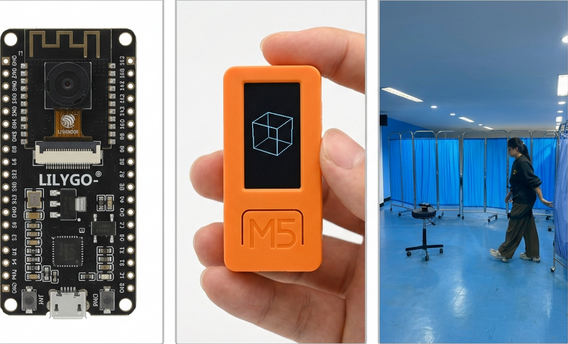
\includegraphics[width=0.65\columnwidth]{hardware_cropped.png}}
\caption{Hardware: (a) ESP32-S3 anchor, (b) M5StickC Plus2 tag, (c) tag on waist.}
\label{fig:hardware}
\vspace{-2mm}
\end{figure}

\subsection{Experimental Design}
\label{sec:expdesign}

\textbf{Case~1: Body Orientation Detection.}
The researcher stands stationary in Zone~D, facing four cardinal directions at two distances ($\leq$1~m, $>$1~m). Classes: Facing~in~(0) and Facing~out~(1)---body blocks the direct path, causing RSSI attenuation~\cite{b6}. Conditions: 4 directions $\times$ 2 distances $\times$ 2 classes $\times$ 3 replicates = 48 episodes; 13 train / 35 test.

\textbf{Case~2: Boundary Transition Detection.}
The researcher stands on demarcation lines between Zone~D and adjacent zones. Binary task: In Zone~D~(0) or Out~(1). Conditions: 2 boundaries $\times$ 2 classes $\times$ 12 replicates = 48 episodes; 13 train / 35 test. This task is \textit{inherently difficult}: cloth partitions provide negligible RF attenuation at 2.4~GHz.

\textbf{Case~3: Multi-Zone Trajectory.}
The researcher walks through all four zones in randomized sequences (e.g., D$\to$C$\to$B$\to$A), pausing 5--6~s per zone. Conditions: 4 zones $\times$ 4 starting positions $\times$ 3 replicates = 48 episodes; 13 train / 35 test. Task: predict exact ordered sequence of zone IDs. \textit{Exact Sequence accuracy} requires all four zone positions to match simultaneously; \textit{Per-Position accuracy} measures the fraction of individual zone positions (out of 4) predicted correctly, independent of other positions in the sequence. LLMs receive the full time series; ML models use four contiguous segments.

\begin{figure*}[!t]
\centerline{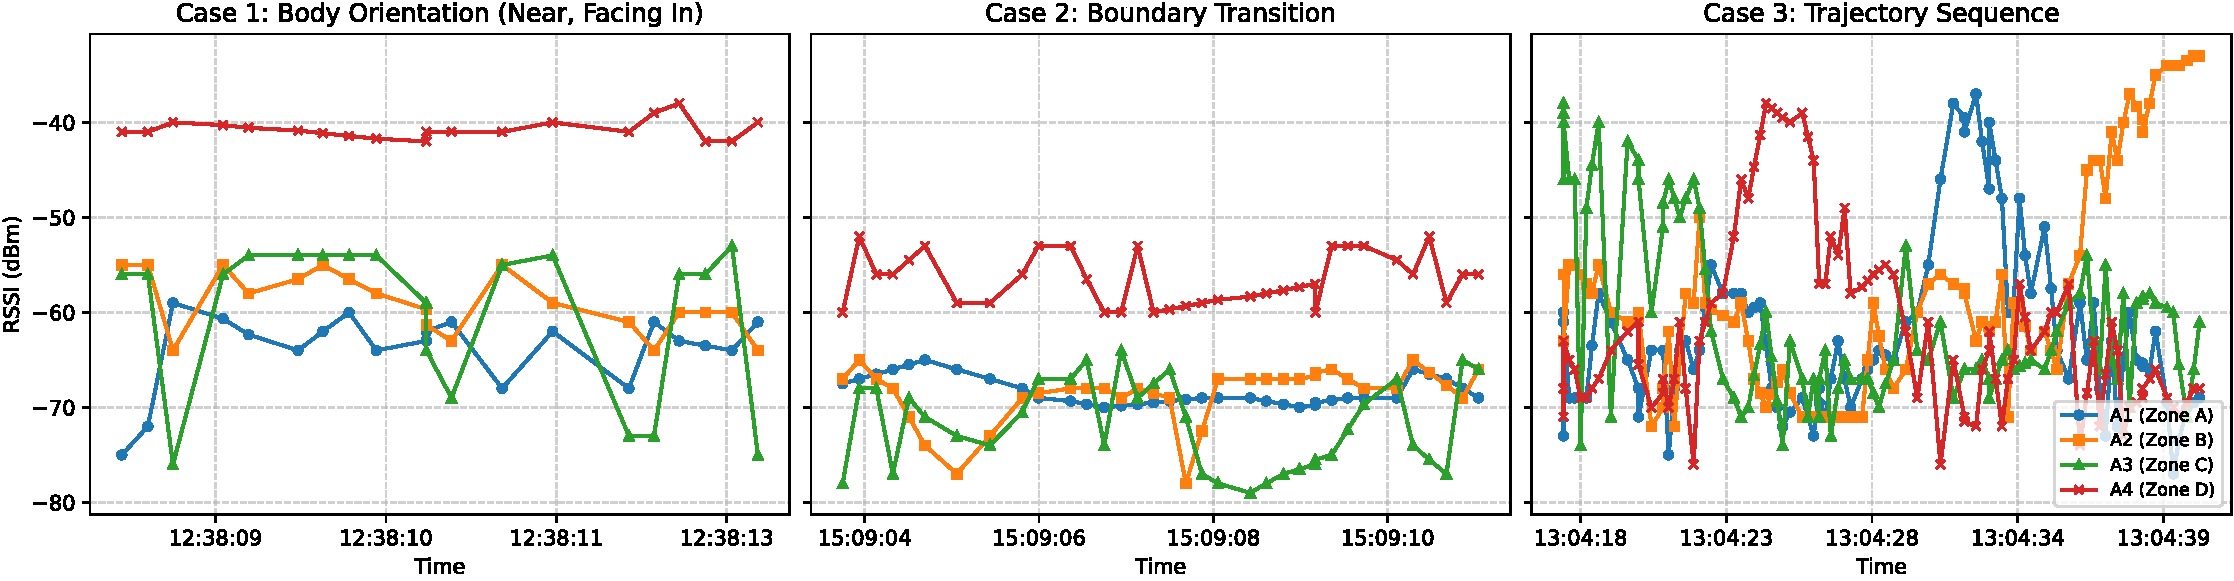
\includegraphics[width=0.9\textwidth]{combined_rssi_plot_fixed.pdf}}
\caption{Example continuous RSSI time-series for Case 1 (Left), Case 2 (Center), and Case 3 (Right).}
\label{fig:combined_rssi_plot}
\end{figure*}

\subsection{Data Collection}
Each case comprises 48 episodes. An \textit{episode} is one continuous recording under fixed experimental conditions, lasting approximately 5~seconds. The dataset is split into 13 training and 35 test episodes by a single random draw without replacement; the same split is used for all models. Raw RSSI values from the four anchors form a 4-dimensional feature vector at each time step, recorded as \texttt{(timestamp)}, \texttt{(r1)}, \texttt{(r2)}, \texttt{(r3)}, \texttt{(r4)} where \texttt{(r1)}--\texttt{(r4)} are the RSSI readings (in dBm) from anchors~1--4 and \texttt{(timestamp)} is the Unix epoch in milliseconds. Missing RSSI readings were forward-filled; no smoothing or filtering was applied to preserve the raw signal dynamics.

\subsection{Machine Learning Models for Classification}

\textbf{KNN} ($k$=5, Euclidean distance): A distance-based classifier applied to per-sample 4D RSSI vectors. For Cases~1 and~2, the episode prediction is obtained by \texttt{round(mean(predictions))}---a soft vote over time steps. For Case~3, each episode is divided into four contiguous segments, and 8D features (mean and standard deviation per anchor per segment) are used for 4-class zone classification.

\textbf{XGBoost} (100 trees, max depth~6, learning rate~0.1): A gradient boosting decision tree model trained on the same features and episode-level aggregation as KNN. Hyperparameters were selected based on commonly used defaults in RSSI fingerprinting studies.

\subsection{Large Language Models for Classification}
\label{sec:prompts}

\textbf{Claude Opus 4.6 and Gemini 3.1 Pro}: Both LLMs receive the raw RSSI time series from test episodes via a task-specific prompt. No training data or labels are provided---predictions are entirely \textit{zero-shot}. Each LLM receives the identical prompt and test CSV. This design reflects typical RSSI fingerprinting pipelines where ML models operate on engineered statistical features, while LLMs process raw sequences.

To ensure reproducibility, prompt formulations for both LLMs were tightly controlled. The design enforces strict zero-shot inference: models receive the task description, class definitions, and input data format without any few-shot examples, domain-specific hints, or physical layout descriptions.

\textbf{Case~1 prompt:} ``\textit{You are acting as an expert indoor motion tracking system. Predict labels for the provided BLE RSSI test dataset (Case~1). Each row in the attached CSV represents one episode. Based only on the RSSI time series data, classify whether the researcher was Facing~in~(0) or Facing~out~(1). Do not provide explanations. Output strictly a Markdown table with two columns: `id' and `predicted'.}'' 

\textbf{Case~2 prompt:} ``\textit{You are acting as an expert indoor motion tracking system. Predict labels for the provided BLE RSSI test dataset (Case~2). Each row in the attached CSV represents one episode. Based only on the RSSI time series data, classify the boundary transition: In zone~4~(0) or Out zone~4~(1). Do not provide explanations. Output strictly a Markdown table with two columns: `id' and `predicted'.}'' 

\textbf{Case~3 prompt:} ``\textit{You are acting as an expert indoor motion tracking system. Predict the trajectory sequence for the provided BLE RSSI test dataset (Case~3). The environment is a single room divided into 4 equal-sized zones (4$\times$4~m each, separated by cloth partitions). Based only on the continuous RSSI time series, predict the exact sequence of 4 zone IDs (1, 2, 3, or 4) visited in order. Example format: `4 3 2 1'. Do not provide explanations. Output strictly a Markdown table with two columns: `id' and `predicted'.}''

The input CSV files format each row as \texttt{experiment\_id} followed by a semicolon-separated list of temporal readings \texttt{timestamp,r1,r2,r3,r4} (RSSI values in dBm). For the robustness evaluation (Section~\ref{sec:robust}), the identical prompts were deployed with altered CSV data; the models were intentionally left uninformed regarding the injected Gaussian noise or anchor failures.

\section{Results and Discussion}

This section evaluates classifier performance across three BLE RSSI motion tracking tasks. We compare two trained ML models (KNN, XGBoost) against two zero-shot LLM classifiers (Claude Opus 4.6, Gemini 3.1 Pro) using accuracy, precision, recall, and F1-score as metrics. Table~\ref{tab:accuracy} summarizes performance across all three cases (35 test episodes each). Tables~\ref{tab:cm_case1} and~\ref{tab:cm_case2} present the confusion matrices for the binary classification tasks.

\begin{table}[htbp]
\caption{Classification Performance (\%, $n$=35)}
\begin{center}
\begin{tabular}{|c|c|c|c|c|}
\hline
\textbf{Model} & \textbf{Acc.} & \textbf{Prec.} & \textbf{Rec.} & \textbf{F1} \\
\hline
\multicolumn{5}{|l|}{\textit{Case 1: Body Orientation (Facing In/Out)}} \\
\hline
KNN            & 88.57 & 84.21 & 94.12 & 88.89 \\
\hline
XGBoost        & \textbf{97.14} & \textbf{100.00} & 94.12 & \textbf{96.97} \\
\hline
Claude Opus 4.6 & \textbf{97.14} & \textbf{100.00} & 94.12 & \textbf{96.97} \\
\hline
Gemini 3.1 Pro  & 94.29 & 94.12 & 94.12 & 94.12 \\
\hline
\multicolumn{5}{|l|}{\textit{Case 2: Boundary Transition (In/Out Zone D)}} \\
\hline
KNN            & \textbf{68.57} & \textbf{68.75} & 64.71 & \textbf{66.67} \\
\hline
XGBoost        & 57.14 & 54.55 & \textbf{70.59} & 61.54 \\
\hline
Claude Opus 4.6 & 62.86 & 64.29 & 52.94 & 58.06 \\
\hline
Gemini 3.1 Pro  & 34.29 & 36.36 & 47.06 & 41.03 \\
\hline
\multicolumn{5}{|l|}{\textit{Case 3: Trajectory (Exact Seq. / Per-Position)}} \\
\hline
KNN            & 88.57 & \multicolumn{3}{c|}{Per-pos: 97.14} \\
\hline
XGBoost        & 48.57 & \multicolumn{3}{c|}{Per-pos: 85.00} \\
\hline
Claude Opus 4.6 & 94.29 & \multicolumn{3}{c|}{Per-pos: 98.57} \\
\hline
Gemini 3.1 Pro  & \textbf{97.14} & \multicolumn{3}{c|}{Per-pos: \textbf{98.57}} \\
\hline
\end{tabular}
\label{tab:accuracy}
\end{center}
\end{table}

\begin{table}[htbp]
\vspace{-2mm}
\caption{Confusion Matrix --- Case~1 ($n$=35)}
\vspace{-2mm}
\begin{center}
\scriptsize
\resizebox{\columnwidth}{!}{%
\begin{tabular}{|l|cc|cc|cc|cc|}
\hline
 & \multicolumn{2}{c|}{\textbf{KNN}} & \multicolumn{2}{c|}{\textbf{XGBoost}} & \multicolumn{2}{c|}{\textbf{Claude}} & \multicolumn{2}{c|}{\textbf{Gemini}} \\
 & P\,0 & P\,1 & P\,0 & P\,1 & P\,0 & P\,1 & P\,0 & P\,1 \\
\hline
A\,0 & TN=15 & FP=3 & TN=18 & FP=0 & TN=18 & FP=0 & TN=17 & FP=1 \\
A\,1 & FN=1  & TP=16 & FN=1  & TP=16 & FN=1  & TP=16 & FN=1  & TP=16 \\
\hline
\end{tabular}%
}
\label{tab:cm_case1}
\end{center}

\vspace{1mm}
\caption{Confusion Matrix --- Case~2 ($n$=35)}
\vspace{-2mm}
\begin{center}
\scriptsize
\resizebox{\columnwidth}{!}{%
\begin{tabular}{|l|cc|cc|cc|cc|}
\hline
 & \multicolumn{2}{c|}{\textbf{KNN}} & \multicolumn{2}{c|}{\textbf{XGBoost}} & \multicolumn{2}{c|}{\textbf{Claude}} & \multicolumn{2}{c|}{\textbf{Gemini}} \\
 & P\,0 & P\,1 & P\,0 & P\,1 & P\,0 & P\,1 & P\,0 & P\,1 \\
\hline
A\,0 & TN=13 & FP=5 & TN=8  & FP=10 & TN=13 & FP=5 & TN=4  & FP=14 \\
A\,1 & FN=6  & TP=11 & FN=5  & TP=12 & FN=8  & TP=9  & FN=9  & TP=8  \\
\hline
\end{tabular}%
}
\label{tab:cm_case2}
\end{center}
\vspace{-2mm}
\end{table}

\begin{figure}[htbp]
\centerline{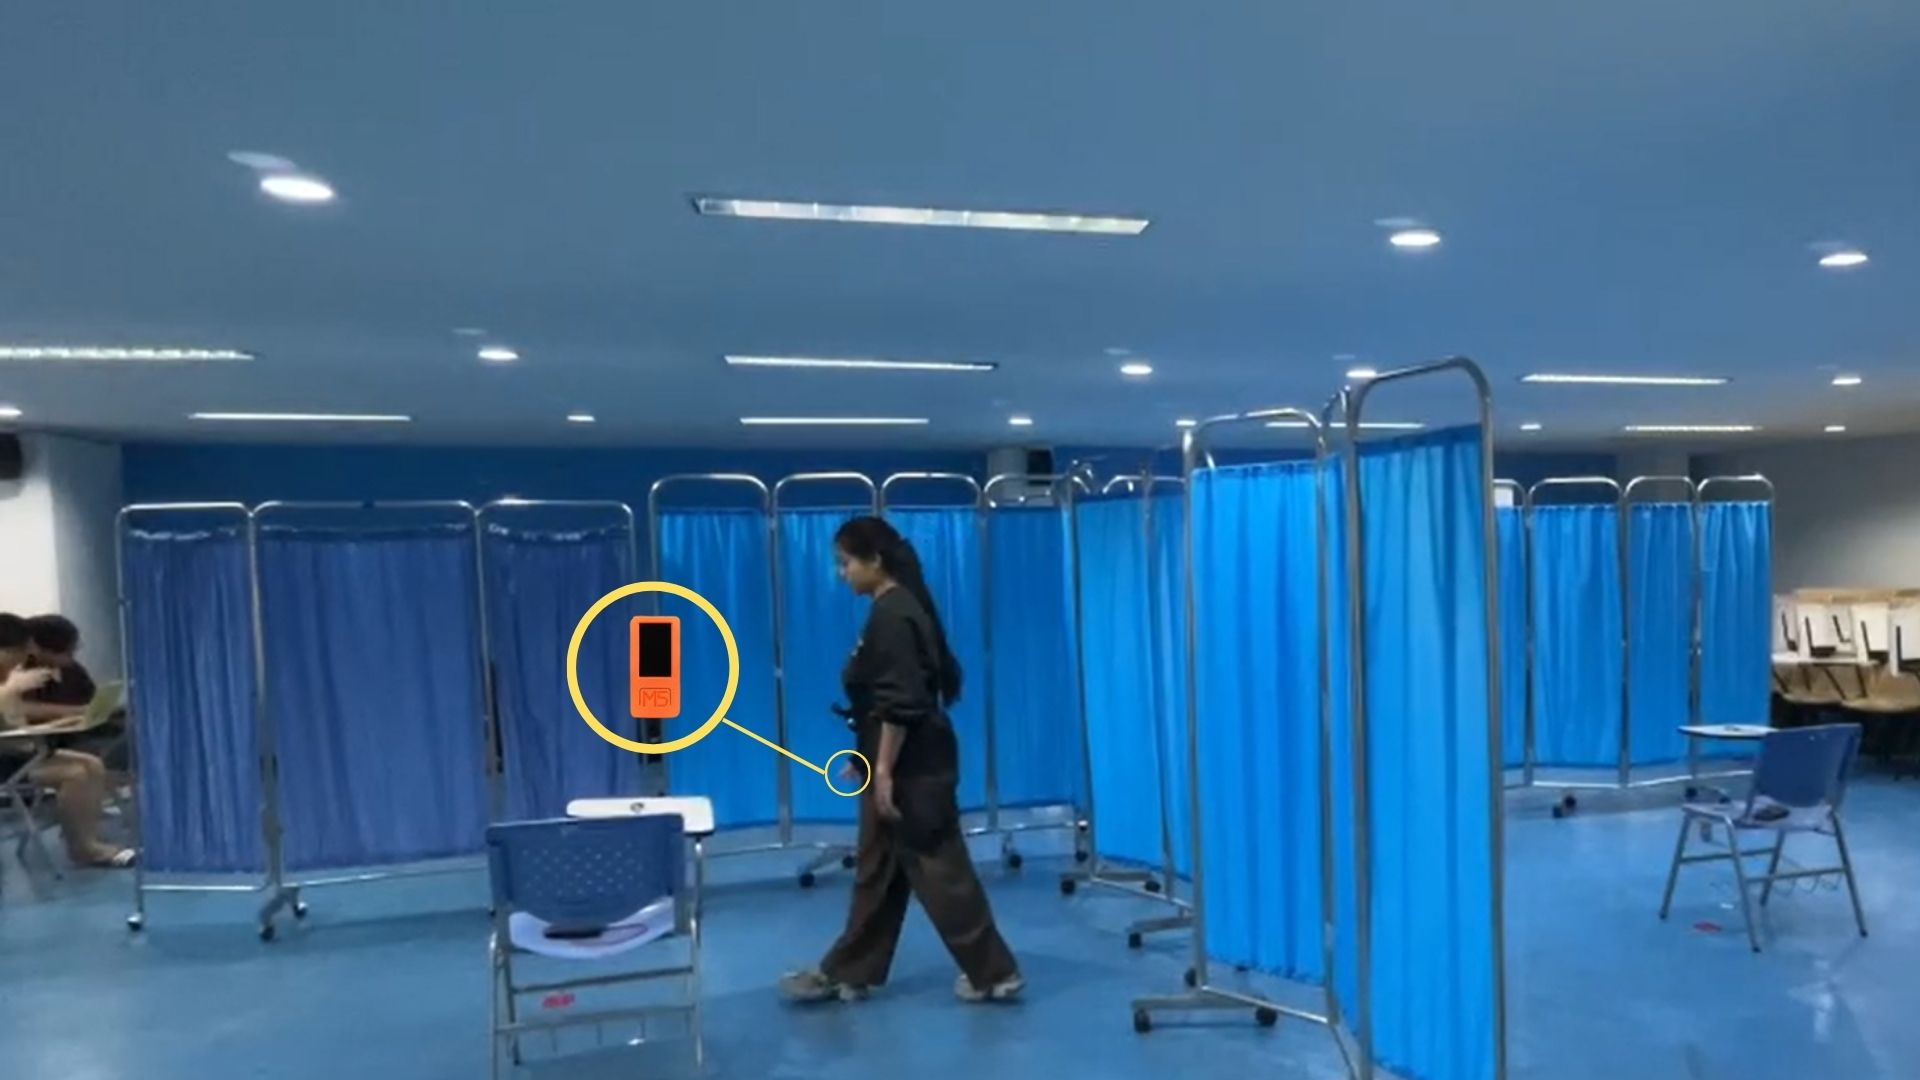
\includegraphics[width=0.65\columnwidth]{validation.jpg}}
\caption{Ground truth video frame showing researcher position.}
\label{fig:validation}
\vspace{-2mm}
\end{figure}

\subsection{Case-by-Case Analysis}

\textbf{Case~1 --- Body Orientation.}
All four models exceed 88\% accuracy, confirming a readily detectable RSSI signature from body shadowing. Body orientation introduces body-shadowing, which significantly attenuates RSSI signals~\cite{b6}. This produces consistent patterns that both ML and LLM models can capture reliably. Both Claude and XGBoost achieve 97.14\% (34/35), each with TN=18, FP=0, FN=1, TP=16. KNN produces 3~FP due to RSSI overlap at boundary distances. Gemini achieves 94.29\% with a balanced error profile (FP=1, FN=1). The consistent RSSI level-shift over a 5-second window~\cite{b6},~\cite{b14} makes this task well-suited to both gradient boosting and zero-shot reasoning.

\textbf{Case~2 --- Boundary Transition.}
This proves the most challenging scenario (Table~\ref{tab:cm_case2}). KNN leads at 68.57\%, followed by Claude (62.86\%), XGBoost (57.14\%), and Gemini (34.29\%---below chance). The difficulty is fundamentally physical: with only one anchor per zone, the system lacks spatial redundancy to resolve boundary positions~\cite{b14}. Body shadowing at boundaries affects all four anchor readings simultaneously~\cite{b6}, creating overlapping RSSI distributions that no classifier can cleanly separate. KNN outperforms XGBoost due to its non-parametric, instance-based nature~\cite{b15}: as an unsupervised-style learner that stores all training instances and performs post-hoc label assignment via distance-weighted voting~\cite{b3}, KNN adapts flexibly to \textit{local} RSSI decision surfaces. This flexibility is particularly advantageous when boundary RSSI distributions are irregularly shaped and position-dependent. XGBoost, by contrast, builds fixed tree splits optimized for globally separable features~\cite{b16}; when boundary RSSI distributions overlap heavily, its axis-aligned decision boundaries cannot capture these subtle, position-specific patterns. Cover and Hart~\cite{b15} demonstrated that instance-based methods achieve near-optimal performance precisely in domains with complex, non-linear decision surfaces. Zero-shot LLMs lack any access to the training distribution, placing them at a structural disadvantage on this ambiguous task.

\textbf{Case~3 --- Multi-Zone Trajectory.}
Gemini achieves 97.14\% (34/35) and Claude reaches 94.29\% (33/35), both substantially outperforming KNN (88.57\%) and XGBoost (48.57\%). The advantage lies in the LLMs' \textit{temporal signal reasoning}---recognizing RSSI peak transitions between anchors as zone changes. Unlike XGBoost, which builds fixed decision trees on per-segment statistics~\cite{b16}, and KNN, which evaluates each segment independently~\cite{b15}, LLMs process the \textit{entire RSSI time series} in a single inference pass. This enables detection of outlier time steps and cross-episode pattern correction that per-sample ML classification cannot achieve. Zhou et al.~\cite{b17} demonstrated that pretrained language models can capture temporal dependencies in time-series data more effectively than traditional segment-based approaches. XGBoost's 85\% per-position accuracy compounds to only $0.85^4 \approx 52\%$ exact-sequence accuracy.


\subsection{Cross-Case Analysis}
A consistent pattern emerges: \textit{LLMs excel when signal patterns are physically distinctive or when temporal reasoning is required} (Cases~1 and~3), whereas \textit{trained ML models prove more robust when signal boundaries are ambiguous} (Case~2). This aligns with theoretical expectations: KNN and XGBoost optimize discriminative boundaries from labeled examples~\cite{b15},~\cite{b16}, whereas LLMs perform inductive reasoning from the full context window~\cite{b17}. Syafri et al.~\cite{b5} similarly observed that ML algorithm performance in BLE RSSI localization varies significantly depending on signal separability, supporting our finding that physical boundary characteristics---rather than model architecture---dominate classification difficulty. Claude demonstrates stronger performance on binary tasks, while Gemini excels at sequential reasoning. The nearly 29-percentage-point gap between Case~2 (KNN: 68.57\%) and Cases~1/3 ($\geq$94\%) underscores this observation.

\begin{figure}[htbp]
\centerline{
\begin{tikzpicture}[scale=0.45, transform shape]
% Axes -- full 0-100% range
\draw[->] (0,0) -- (10.5,0);
\draw[->] (0,0) -- (0,4.5) node[above, font=\scriptsize] {Accuracy (\%)};
\foreach \y/\lbl in {0/0, 1/25, 2/50, 3/75, 4/100} {
    \draw (0,\y) -- (-0.15,\y) node[left, font=\scriptsize] {\lbl};
    \draw[dotted, gray!40] (0,\y) -- (10.3,\y);
}
% Case 1 bars (val/100*4)
\node[font=\scriptsize\bfseries] at (1.65,-0.7) {Case 1};
\fill[blue!70] (0.5,0) rectangle (1.0,3.543);     % KNN 88.57
\fill[orange!80] (1.1,0) rectangle (1.6,3.886);     % XGB 97.14
\fill[green!70] (1.7,0) rectangle (2.2,3.886);    % Claude 97.14
\fill[red!70] (2.3,0) rectangle (2.8,3.771); % Gemini 94.29
% Case 2 bars
\node[font=\scriptsize\bfseries] at (4.95,-0.7) {Case 2};
\fill[blue!70] (3.8,0) rectangle (4.3,2.743);     % KNN 68.57
\fill[orange!80] (4.4,0) rectangle (4.9,2.286);     % XGB 57.14
\fill[green!70] (5.0,0) rectangle (5.5,2.514);    % Claude 62.86
\fill[red!70] (5.6,0) rectangle (6.1,1.371); % Gemini 34.29
% Case 3 bars
\node[font=\scriptsize\bfseries] at (8.25,-0.7) {Case 3};
\fill[blue!70] (7.1,0) rectangle (7.6,3.543);     % KNN 88.57
\fill[orange!80] (7.7,0) rectangle (8.2,1.943);     % XGB 48.57
\fill[green!70] (8.3,0) rectangle (8.8,3.771);    % Claude 94.29
\fill[red!70] (8.9,0) rectangle (9.4,3.886); % Gemini 97.14
% Legend
\fill[blue!70] (1.5,4.7) rectangle (1.8,4.9); \node[font=\scriptsize, right] at (1.85,4.8) {KNN};
\fill[orange!80] (3.5,4.7) rectangle (3.8,4.9); \node[font=\scriptsize, right] at (3.85,4.8) {XGBoost};
\fill[green!70] (5.8,4.7) rectangle (6.1,4.9); \node[font=\scriptsize, right] at (6.15,4.8) {Claude};
\fill[red!70] (8.2,4.7) rectangle (8.5,4.9); \node[font=\scriptsize, right] at (8.55,4.8) {Gemini};
\end{tikzpicture}
}
\caption{Accuracy comparison across three cases.}
\label{fig:comparison}
\vspace{-2mm}
\end{figure}


\subsection{LLM Reasoning Process Analysis}
\label{sec:reasoning}

A distinctive advantage of LLM-based classifiers lies in their ability to reason over the entire input dataset in a single inference pass. Traditional ML models are \textit{stateless}: KNN and XGBoost apply a fixed function to each feature vector independently~\cite{b15},~\cite{b16}. LLMs operate over a full context window encompassing the entire test set, enabling them to identify recurring patterns, detect outliers, and leverage cross-episode consistency. Zhou et al.~\cite{b17} demonstrated that pretrained language models possess inherent temporal pattern recognition capabilities that transfer effectively to structured numerical data.

Chain-of-thought (CoT) reasoning~\cite{b18} traces reveal that LLMs spontaneously execute structured analytical workflows: feature identification, pattern discovery, cluster validation, and self-correction. Wei et al.~\cite{b18} showed that this emergent step-by-step reasoning significantly improves performance on complex analytical tasks. Case~3 traces show even more sophisticated behavior---the LLM evaluates multiple segmentation strategies, constructs state transition models, and proactively verifies edge cases.

The effectiveness stems from three factors: (i)~BLE RSSI exhibits \textit{physically grounded patterns}---stronger signal implies proximity~\cite{b6}; (ii)~the data is compact, fitting within the model's working memory; and (iii)~the task maps to \textit{comparative reasoning} across anchors~\cite{b7},~\cite{b8}.



\section{Robustness Under Signal Degradation}
\label{sec:robust}
Two offline experiments evaluate robustness: (1)~Gaussian noise injection ($\sigma$ = 2--12~dBm) added to each RSSI sample, and (2)~simulated anchor failure by replacing 1 or 2 anchors with $-$100~dBm. The same prompts from Section~\ref{sec:prompts} are reused without modification.

\subsection{Noise Resilience}
Table~\ref{tab:noise_all} shows accuracy under increasing noise. ML fluctuations (e.g., KNN Case~1 rising at $\sigma$=2) are expected with stochastic noise and $n$=35. In Case~1, all models maintain $>$77\% accuracy at $\sigma$=12~dBm, confirming that the body-shadowing signal margin exceeds typical indoor noise levels~\cite{b14}. Kaemarungsi and Krishnamurthy~\cite{b14} demonstrated that RSSI-based systems can tolerate moderate noise levels when underlying signal patterns are sufficiently distinctive. Claude degrades 12~pp (97.14$\to$85.71\%), Gemini 17~pp, while ML models show non-monotonic fluctuations due to stochastic effects with $n$=35.

In Case~3, LLMs demonstrate superior noise resilience: at $\sigma$=12, Claude (74.29\%) and Gemini (82.86\%) both outperform the ML \textit{baselines at $\sigma$=0} (KNN: 57.14\%, XGBoost: 45.71\%), indicating that temporal reasoning over the full time series provides inherent noise tolerance that per-sample classification cannot achieve~\cite{b17}. Case~2 shows minimal additional degradation from noise across all models, confirming that boundary-task difficulty is dominated by the physical ambiguity of cloth partitions rather than signal noise~\cite{b5}.

\begin{table}[htbp]
\caption{Accuracy Under Gaussian Noise (\%)}
\begin{center}
\scriptsize
\begin{tabular}{|c|c|cc|cc|}
\hline
\textbf{Case} & $\sigma$ & \textbf{KNN} & \textbf{XGB} & \textbf{Claude} & \textbf{Gemini} \\
\hline
\multirow{7}{*}{1}
 & 0  & 88.57 & 97.14 & 97.14 & 94.29 \\
 & 2  & 91.43 & 97.14 & 88.57 & 91.43 \\
 & 4  & 88.57 & 100.00 & 88.57 & 91.43 \\
 & 6  & 91.43 & 97.14 & 85.71 & 88.57 \\
 & 8  & 85.71 & 94.29 & 85.71 & 82.86 \\
 & 10 & 94.29 & 94.29 & 88.57 & 85.71 \\
 & 12 & 85.71 & 82.86 & 85.71 & 77.14 \\
\hline
\multirow{7}{*}{2}
 & 0  & 68.57 & 57.14 & 62.86 & 34.29 \\
 & 2  & 68.57 & 54.29 & 60.00 & 31.43 \\
 & 4  & 71.43 & 62.86 & 57.14 & 34.29 \\
 & 6  & 60.00 & 62.86 & 54.29 & 28.57 \\
 & 8  & 60.00 & 65.71 & 51.43 & 31.43 \\
 & 10 & 60.00 & 51.43 & 48.57 & 25.71 \\
 & 12 & 62.86 & 62.86 & 45.71 & 25.71 \\
\hline
\multirow{7}{*}{3}
 & 0  & 57.14 & 45.71 & 94.29 & 97.14 \\
 & 2  & 60.00 & 34.29 & 91.43 & 97.14 \\
 & 4  & 62.86 & 34.29 & 88.57 & 97.14 \\
 & 6  & 54.29 & 37.14 & 85.71 & 91.43 \\
 & 8  & 62.86 & 28.57 & 82.86 & 91.43 \\
 & 10 & 54.29 & 40.00 & 80.00 & 85.71 \\
 & 12 & 51.43 & 22.86 & 74.29 & 82.86 \\
\hline
\end{tabular}
\label{tab:noise_all}
\end{center}
\end{table}

\subsection{Anchor Failure}
Table~\ref{tab:anchor_failure} shows accuracy when 1 or 2 anchors fail. ML models are deterministic: their predictions for identical input are reproducible at negligible computational cost, so ML accuracy is averaged exhaustively over all $\binom{4}{k}$ anchor failure combinations ($k$=1 or 2). LLM inference, however, requires individual API calls with 1--3~minute latency per episode set, making exhaustive evaluation over all combinations prohibitively expensive. Accordingly, LLM results report a single representative combination selected by removing the anchor(s) closest to the tag's primary zone, representing the most informative failure scenario.

In Case~1, Claude retains 91.43\% accuracy even with 2~anchors lost, while KNN drops to 56.67\% ($-$32~pp) and XGBoost to 70.95\% ($-$26~pp). This occurs because ML models' fixed 4D feature space is fundamentally disrupted when dimensions are replaced with $-$100~dBm, whereas the LLM processes the time series as text and can adaptively ignore anomalous channels. This behavior parallels the LLM context-filtering capability described by Gruver et al.~\cite{b8}---the model down-weights obviously corrupted channels without being explicitly instructed to do so. Case~3 reveals the largest ML--LLM gap under degradation: with 2~anchors lost, KNN drops to 4.29\% ($-$53~pp), XGBoost to 9.05\% ($-$37~pp), while Claude retains 62.86\% ($-$31~pp) and Gemini 68.57\% ($-$29~pp). Zhou et al.~\cite{b17} attributed this resilience to pretrained language models' ability to identify and down-weight corrupted input segments through contextual attention mechanisms.

\begin{table}[htbp]
\caption{Accuracy Under Anchor Failure (\%)}
\begin{center}
\begin{tabular}{|c|c|cc|cc|}
\hline
\textbf{Case} & \textbf{Cond.} & \textbf{KNN} & \textbf{XGB} & \textbf{Claude} & \textbf{Gemini} \\
\hline
\multirow{3}{*}{1}
 & All 4  & 88.57 & 97.14 & 97.14 & 94.29 \\
 & 1 lost & 75.71 & 84.29 & 94.29 & 85.71 \\
 & 2 lost & 56.67 & 70.95 & 91.43 & 74.29 \\
\hline
\multirow{3}{*}{2}
 & All 4  & 68.57 & 57.14 & 62.86 & 34.29 \\
 & 1 lost & 51.43 & 65.71 & 54.29 & 31.43 \\
 & 2 lost & 50.00 & 65.71 & 48.57 & 28.57 \\
\hline
\multirow{3}{*}{3}
 & All 4  & 57.14 & 45.71 & 94.29 & 97.14 \\
 & 1 lost & 15.00 & 24.29 & 80.00 & 85.71 \\
 & 2 lost & 4.29  & 9.05  & 62.86 & 68.57 \\
\hline
\end{tabular}
\label{tab:anchor_failure}
\end{center}
\vspace{-4mm}
\end{table}

\section{Conclusion}

This study compares trained ML classifiers (KNN, XGBoost) against zero-shot LLM classifiers (Claude Opus 4.6, Gemini 3.1 Pro) for BLE RSSI-based indoor motion tracking.

\textbf{Key findings.} LLMs excel when temporal reasoning or distinctive signal patterns are present: Gemini achieves 97.14\% exact-sequence accuracy in trajectory prediction (Case~3), and Claude matches XGBoost at 97.14\% for body orientation (Case~1). For the ambiguous boundary transition task (Case~2), KNN's instance-based flexibility achieves 68.57\%, surpassing all other models. This demonstrates that physical signal separability---not model sophistication---determines classification accuracy.

\textbf{Robustness.} LLMs show marked advantage under hardware degradation. Claude retains 91.43\% with two anchors lost in Case~1, versus KNN's 56.67\%. In Case~3 with two anchors failed, LLMs maintain $>$62\% while ML models drop below 10\%, indicating that full time-series reasoning provides inherent fault tolerance.

\textbf{Practical implications.} ML models offer sub-10~ms edge inference, while LLM API calls require 1--3~minutes. This suggests a hybrid architecture: ML for real-time tracking, with LLMs for offline trajectory reconstruction or when anchor degradation reduces ML accuracy. LLM-based RSSI analysis also offers a privacy-preserving alternative to CCTV for healthcare environments.

\textbf{Limitations and future work.} The dataset comprises only 48~episodes per case (35~test), yielding a resolution of 2.86~pp per episode; accuracy differences below approximately $\pm$12~pp should therefore be interpreted with caution. All experiments are conducted in a single controlled room with cloth partitions, which limits generalizability to diverse real-world settings such as multi-room buildings with solid walls and varying materials. Additionally, the ML baselines (KNN, XGBoost) treat each segment independently; recurrent architectures such as RNN or LSTM could process the raw Case~3 time series directly without segment-based aggregation, potentially narrowing the ML--LLM accuracy gap on trajectory prediction. The current analysis is primarily empirical; a formal theoretical framework characterizing the conditions under which zero-shot LLM reasoning outperforms trained classifiers---in terms of signal separability, temporal structure, and context length---would strengthen the contributions. Future work includes validation in diverse environments with solid walls and multi-floor layouts, evaluation with larger datasets, few-shot learning for boundary transitions, temporal ML baselines (RNN, LSTM, Transformer-based models), and on-device compact language models for real-time inference.


\ifblindreview
\section*{Acknowledgment}
\noindent\blind{\parbox{\dimexpr\columnwidth-2\fboxsep\relax}{The authors thank the Thammasat School of Engineering and the CED-Square Innovation Center for providing the research facilities, equipment, and support that made this work possible.}}
\else
\section*{Acknowledgment}
The authors thank the Thammasat School of Engineering and the CED-Square Innovation Center for providing the research facilities, equipment, and support that made this work possible.
\fi

\begin{thebibliography}{00}
\bibitem{b1} A. Yassin \textit{et al.}, ``Recent Advances in Indoor Localization: A Survey on Theoretical Approaches and Applications,'' \textit{IEEE Commun. Surv. Tuts.}, vol.~19, no.~2, pp.~1327--1346, 2017.
\bibitem{b2} P. Spachos and K. N. Plataniotis, ``BLE Beacons for Indoor Positioning at an Interactive IoT-Based Smart Museum,'' \textit{IEEE Syst. J.}, vol.~14, no.~3, pp.~3483--3493, 2020.
\bibitem{b3} S. He and S.-H. G. Chan, ``Wi-Fi Fingerprint-Based Indoor Positioning: Recent Advances and Comparisons,'' \textit{IEEE Commun. Surv. Tuts.}, vol.~18, no.~1, pp.~466--490, 2016.
\bibitem{b4} Y. Li \textit{et al.}, ``Two-Step XGBoost Model for Indoor Localization Using RSSI,'' \textit{IEEE Access}, vol.~8, pp.~47528--47541, 2020.
\bibitem{b5} A. F. Syafri, S. Yuliana, and R. Arifuddin, ``Comparative Analysis of Machine Learning Algorithms for BLE RSSI-Based Indoor Localization,'' \textit{Proc. IEEE Int. Conf. Commun., Netw. Satell. (COMNETSAT)}, pp.~142--148, 2023.
\bibitem{b6} D. Giovanelli \textit{et al.}, ``Bluetooth-Based Indoor Positioning Through Angle of Arrival Estimation: Body Shadowing Compensation and Performance Analysis,'' \textit{IEEE Trans. Instrum. Meas.}, vol.~70, pp.~1--12, 2021.
\bibitem{b7} M. Jin \textit{et al.}, ``Time-LLM: Time Series Forecasting by Reprogramming Large Language Models,'' \textit{Proc. Int. Conf. Learn. Representations (ICLR)}, 2024.
\bibitem{b8} N. Gruver \textit{et al.}, ``Large Language Models Are Zero-Shot Time Series Forecasters,'' \textit{Proc. Adv. Neural Inf. Process. Syst. (NeurIPS)}, vol.~36, 2023.
\bibitem{b9} F. Zafari, A. Gkelias, and K. K. Leung, ``A Survey of Indoor Localization Systems and Technologies,'' \textit{IEEE Commun. Surv. Tuts.}, vol.~21, no.~3, pp.~2550--2599, 2019.
\bibitem{b10} P. Bahl and V. N. Padmanabhan, ``RADAR: An In-Building RF-Based User Location and Tracking System,'' \textit{Proc. IEEE INFOCOM}, pp.~775--784, 2000.
\bibitem{b11} R. Faragher and R. Harle, ``Location Fingerprinting with Bluetooth Low Energy Beacons,'' \textit{IEEE J. Sel. Areas Commun.}, vol.~33, no.~11, pp.~2418--2428, 2015.
\bibitem{b12} K. S. Ahn and O. S. Shin, ``Deep Learning-Based Indoor Localization Using Wi-Fi RSSI,'' \textit{IEEE Access}, vol.~9, pp.~141852--141865, 2021.
\bibitem{b13} T. S. Rappaport, \textit{Wireless Communications: Principles and Practice}, 2nd ed. Prentice Hall, 2001.
\bibitem{b14} K. Kaemarungsi and P. Krishnamurthy, ``Analysis of WLAN's Received Signal Strength Indication for Indoor Location Fingerprinting,'' \textit{Pervasive Mobile Comput.}, vol.~8, no.~2, pp.~292--316, 2012.
\bibitem{b15} T. M. Cover and P. E. Hart, ``Nearest Neighbor Pattern Classification,'' \textit{IEEE Trans. Inf. Theory}, vol.~13, no.~1, pp.~21--27, 1967.
\bibitem{b16} T. Chen and C. Guestrin, ``XGBoost: A Scalable Tree Boosting System,'' \textit{Proc. ACM SIGKDD Int. Conf. Knowl. Discov. Data Min.}, pp.~785--794, 2016.
\bibitem{b17} T. Zhou \textit{et al.}, ``One Fits All: Power General Time Series Analysis by Pretrained LM,'' \textit{Proc. Adv. Neural Inf. Process. Syst. (NeurIPS)}, vol.~36, 2023.
\bibitem{b18} J. Wei \textit{et al.}, ``Chain-of-Thought Prompting Elicits Reasoning in Large Language Models,'' \textit{Proc. Adv. Neural Inf. Process. Syst. (NeurIPS)}, vol.~35, 2022.
\end{thebibliography}

\end{document}
